%%%%%%%%%%%%%%%%%%%%%%%%%%%%%%%%%%%%%%%%%
% Beamer Presentation
% LaTeX Template
% Version 1.0 (10/11/12)
%
% This template has been downloaded from:
% http://www.LaTeXTemplates.com
%
% License:
% CC BY-NC-SA 3.0 (http://creativecommons.org/licenses/by-nc-sa/3.0/)
%
%%%%%%%%%%%%%%%%%%%%%%%%%%%%%%%%%%%%%%%%%

%----------------------------------------------------------------------------------------
%	PACKAGES AND THEMES
%----------------------------------------------------------------------------------------

\documentclass{beamer}

\mode<presentation> {

% The Beamer class comes with a number of default slide themes
% which change the colors and layouts of slides. Below this is a list
% of all the themes, uncomment each in turn to see what they look like.

%\usetheme{default}
%\usetheme{AnnArbor}
%\usetheme{Antibes}
%\usetheme{Bergen}
%\usetheme{Berkeley}
%\usetheme{Berlin}
%\usetheme{Boadilla}
%\usetheme{CambridgeUS}
%\usetheme{Copenhagen}
%\usetheme{Darmstadt}
%\usetheme{Dresden}
%\usetheme{Frankfurt}
%\usetheme{Goettingen}
%\usetheme{Hannover}
%\usetheme{Ilmenau}
%\usetheme{JuanLesPins}
%\usetheme{Luebeck}
\usetheme{Madrid}
%\usetheme{Malmoe}
%\usetheme{Marburg}
%\usetheme{Montpellier}
%\usetheme{PaloAlto}
%\usetheme{Pittsburgh}
%\usetheme{Rochester}
%\usetheme{Singapore}
%\usetheme{Szeged}
%\usetheme{Warsaw}

% As well as themes, the Beamer class has a number of color themes
% for any slide theme. Uncomment each of these in turn to see how it
% changes the colors of your current slide theme.

%\usecolortheme{albatross}
%\usecolortheme{beaver}
%\usecolortheme{beetle}
%\usecolortheme{crane}
%\usecolortheme{dolphin}
%\usecolortheme{dove}
%\usecolortheme{fly}
%\usecolortheme{lily}
%\usecolortheme{orchid}
%\usecolortheme{rose}
%\usecolortheme{seagull}
%\usecolortheme{seahorse}
%\usecolortheme{whale}
%\usecolortheme{wolverine}

%\setbeamertemplate{footline} % To remove the footer line in all slides uncomment this line
%\setbeamertemplate{footline}[page number] % To replace the footer line in all slides with a simple slide count uncomment this line

%\setbeamertemplate{navigation symbols}{} % To remove the navigation symbols from the bottom of all slides uncomment this line
}
\usepackage[T1]{fontenc}
\usepackage[utf8]{inputenc}
\usepackage{graphicx} % Allows including images
\usepackage{booktabs} % Allows the use of \toprule, \midrule and \bottomrule in tables
% TiKz stuff
\usepackage{caption}
\usepackage{tikz}
\usetikzlibrary{shapes,%
	fit,%
	positioning,%
	arrows,%
	intersections,%
	shadows.blur,%
	chains%
}
\usepackage{subfigure}
\setbeamertemplate{caption}[numbered]


%----------------------------------------------------------------------------------------
%	TITLE PAGE
%----------------------------------------------------------------------------------------

\title[Communications intra et inter cloud]{Communication Machine to Machine sécurisée appliquée aux workflows} % The short title appears at the bottom of every slide, the full title is only on the title page
\author[Constantin DIVRIOTIS]{\textbf {Présenté par : Constantin DIVRIOTIS \\ \footnotesize Encadré par : Andréas GUILLOT}} % Your name
\institute[Unistra] % Your institution as it will appear on the bottom of every slide, may be shorthand to save space
{Equipe réseaux - UFR Mathématique et Informatique -
Université de Strasbourg \\ % Your institution for the title page
\medskip
\textit{constantin.divriotis@etu.unistra.fr} % Your email address
}
\date{15 Mai 2019} % Date, can be changed to a custom date
\titlegraphic{%
	\begin{figure}
		\begin{minipage}{.45\textwidth}
			\centering
			
\includegraphics[width=3cm,keepaspectratio]{./pics/uds.pdf}%
		\end{minipage}
		\begin{minipage}{.45\textwidth}
			\centering
			
\includegraphics[width=2cm,keepaspectratio]{pics/icube.pdf}%
		\end{minipage}
	\end{figure}
}

%------------------------------------------------

%------------------------------------------------

\begin{document}

\begin{frame}
\titlepage % Print the title page as the first slide
\end{frame}

%------------------------------------------------

%------------------------------------------------

\begin{frame}
\frametitle{Overview} % Table of contents slide, comment this block out to remove it
	\begin{figure}
		\centering
		\captionsetup{justification=centering}
		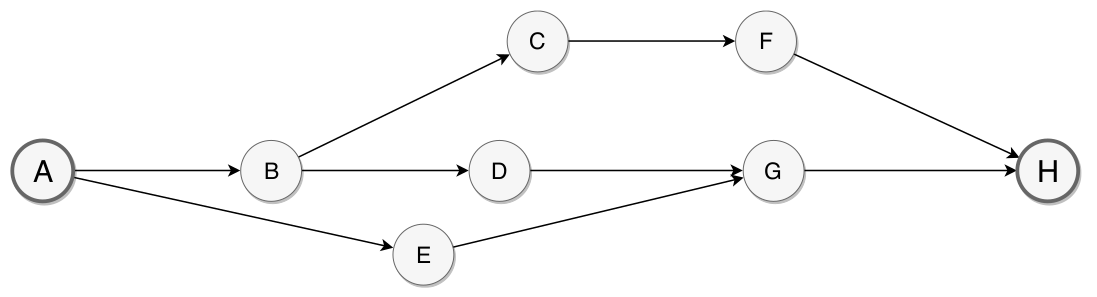
\includegraphics[width=.95\textwidth]{./pics/systeme_workflow.png}
		\caption{Exemple de workflow contenant un ensemble de communications entre différents acteurs}
		\label{figure1}
	\end{figure}
\end{frame}

%------------------------------------------------

%------------------------------------------------


\begin{frame}
\frametitle{Qu'est que le cloud computing ?}

\begin{block}{Définition du NIST}
	\begin{quote}
		Modèle établissant un accès à distance \textcolor{red}{via le réseau, à la demande et en libre-service}, à des ressources informatiques partagées
	configurables
	\end{quote}
\end{block}

\end{frame}

%------------------------------------------------

%------------------------------------------------

\begin{frame}
\frametitle{Sécurité du cloud}
    % L'argument optionnel est utilisé pour centrer tous les items
    \begin{description}[Authentification :]
    \setlength\itemsep{.5cm}
	\item[Disponibilité :] ressources toujours accessibles
	\item[Integrité :] impossible de modifier ou supprimer sans autorisation un fichier
	\item[Confidentialité :] données secrètes
	\item[Contrôle :] gestion des ressources
	\item[Authentification :] garantie l'identité d'un utilisateur
        % La définition de non-rép n'était pas claire, je l'ai donc modifiée
	\item[Non-répudiation :] un utilisateur ne peut pas remettre ses actions en
        cause
\end{description}
\end{frame}

%------------------------------------------------

%------------------------------------------------


\begin{frame}
\frametitle{Enjeux de la sécurité du cloud}
\begin{figure}[h]
	\centering
	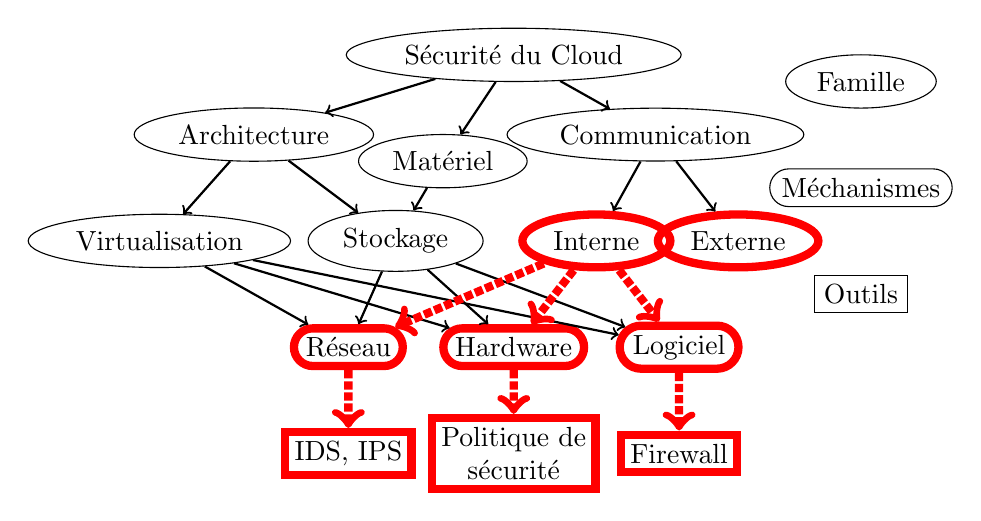
\begin{tikzpicture}[y=-0.9cm, scale=0.75, x=-0.8cm]
	\begin{scope}[every node/.style={ellipse, draw}]
	\node (A) at (-0.5,0.5) {Sécurité du Cloud};
	\node (B) at (-3.5,2) {Communication};
	\node (C) at (5,2) {Architecture};
	\node (HY) at (1, 2.5) {Matériel};
	\node (FA) at (-7.85,1) {Famille};
	\end{scope}
	
	\begin{scope}[every node/.style={ellipse, draw, align=center}]
	\node (H) at (7,4) {Virtualisation};
	\node (J) at (2,4) {Stockage};
	\end{scope}
	\begin{scope}[every node/.style={ellipse, draw=red, align=center, line width=3pt}]
	\node (F) at (-5.25,4) {Externe};
	\node (G) at (-2.25,4) {Interne};
	\end{scope}
	\begin{scope}[every node/.style={fill=white,circle,bottom},
	every path/.style={draw=black, thick}]
	\path [->] (A) -- (B);
	\path [->] (A) -- (C);
	\path [->] (A) -- (HY);
	\path [->] (C) -- (H);
	\path [->] (C) -- (J);
	\path [->] (HY) -- (J);
	\path [->] (B) -- (G);
	\path [->] (B) -- (F);
	
	\end{scope}
	\begin{scope}[every node/.style={draw=red, rounded rectangle, align=center,
		line width=3pt}]
	\node (TR) at (-4,6) {Logiciel};
	\node (LI) at (3,6) {Réseau};
	\node (TI) at (-0.5,6) {Hardware};
	\end{scope}
	\begin{scope}[every node/.style={draw, rounded rectangle, align=center}]
	\node (FA) at (-7.85,3) {Méchanismes};
	\end{scope}
	\begin{scope}[every node/.style={fill=white,circle,bottom},
	every path/.style={draw=black, thick}]
	\path [->] (H) -- (TR);
	\path [->] (H) -- (LI);
	\path [->] (H) -- (TI);
	\path [->] (J) -- (TR);
	\path [->] (J) -- (LI);
	\path [->] (J) -- (TI);
	\end{scope}
	\begin{scope}[every node/.style={fill=white,circle,bottom},
	every path/.style={draw=red, densely dotted, line width=3pt}]
	\path [->] (G) -- (TR);
	\path [->] (G) -- (LI);
	\path [->] (G) -- (TI);
	\end{scope}
	\begin{scope}[every node/.style={draw=red, rectangle, align=center, line width=3pt}]
	\node (ZA) at (3,8) {IDS, IPS};
	\node (ZB) at (-4,8) {Firewall};
	\node (ZC) at (-.5,8) {Politique de\\sécurité};
	\end{scope}
	\begin{scope}[every node/.style={draw, rectangle, align=center}]
	\node (ZZ) at (-7.85,5) {Outils};
	\end{scope}
	\begin{scope}[every node/.style={fill=white,circle,bottom},
	every path/.style={draw=red, densely dotted, line width=3pt}]
	\path [->] (LI) -- (ZA);
	\path [->] (TR) -- (ZB);
	\path [->] (TI) -- (ZC);
	\end{scope}
	\end{tikzpicture}
	\caption{Challenges de la sécurité du cloud}
	\label{figure2}
\end{figure}
\end{frame}

%------------------------------------------------

%------------------------------------------------

\begin{frame}
\frametitle{Enjeux de la sécurité du cloud}
\begin{block}{Problématique}
	Comment obtenir un réseau sécurisé tout en garantissant un niveau de performance élevé et une confiance limitée à tous les
	niveaux ?
\end{block}
\end{frame}

%------------------------------------------------

%------------------------------------------------

\begin{frame}
\frametitle{Cas d'étude : \textit{Tree-Rule firewall}\footnote[frame]{X. He, T. Chomsiri, P. Nanda, Z. Tan, Improving cloud network security using the tree-rule firewall,Future Gener. Comput. Syst. 30 (2014) 116–126}}
\begin{itemize}
	\item Faire respecter la politique de sécurité du réseau
	\item Environnement cloud
	\item \textit{Listed-Rule firewall} présente de gros inconvénients tels que :
		\begin{itemize}
			\item Présence de \textit{Shadowed Rule}
			\item Changements de positions des règles problématiques
			\item Règles redondantes possibles
			\item Configuration difficile
			\item Recherche séquentielle
		\end{itemize}
\end{itemize}
\end{frame}

%------------------------------------------------

%------------------------------------------------

\begin{frame}
\frametitle{Cas d'étude : \textit{Tree-Rule firewall}}
\begin{figure}
	\centering
	\captionsetup{justification=centering}
	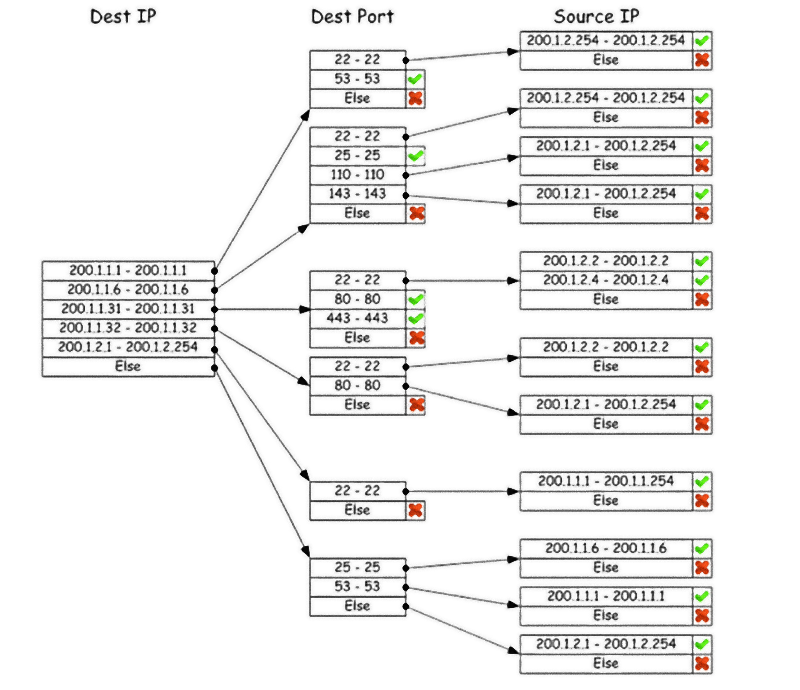
\includegraphics[width=8cm]{./pics/tree_rule_firewall.png}
	\caption{Structure d'un \textit{Tree-Rule firewall}}
	\label{figure3}
\end{figure}
\end{frame}

%------------------------------------------------

%------------------------------------------------

\begin{frame}
\frametitle{Cas d'étude : \textit{Tree-Rule firewall}}
\begin{figure}
	\centering
	\captionsetup{justification=centering}
	\includegraphics[width=12.25cm]{./pics/tableau_comparatif_firewall.png}
	\caption{Comparaison des fonctionnalités de différents firewall dans un environnement cloud}
	\label{figure4}
\end{figure}
\end{frame}

%------------------------------------------------

%------------------------------------------------

\begin{frame}
\frametitle{Conclusion et perspectives}
\begin{block}{Conclusions}
	\begin{itemize}
		\item Le cloud a généré de nouveaux problèmes
		\item Propositions de plusieurs pistes répondant à la problématique
		\item \textit{Tree-Rule firewall} est un exemple
	\end{itemize}
\end{block}
\vfill
\begin{block}{Perspectives}
	\begin{itemize}
		\item Gestion d'IPv6, du NAT ou encore des VPNs dans le \textit{Tree-Rule firewall}
		\item Décalage entre la sécurité mise en place et l'évolution des technologies actuelles, comment y remédier ?
	\end{itemize}
\end{block}
\end{frame}

%------------------------------------------------

%------------------------------------------------

\begin{frame}
\frametitle{References}
\footnotesize{
\begin{thebibliography}{99} % Beamer does not support BibTeX so references must be inserted manually as below
\bibitem[nist_definition, September 2011]{p1} Peter Mell and Timothy Grance (2011)
\newblock The NIST Definition of Cloud Computing
\newblock \emph{NIST Special Publication, 800-145}.

\bibitem[security_survey, June 2015]{p1} Mazhar Ali, Samee U. Khan and Athanasios V. Vasilakos (2015)
\newblock Security in cloud computing: Opportunities and challenges
\newblock \emph{Elsevier : Information Sciences}, 305, 357-383.

\bibitem[tree_rule_firewall, 2014]{p1} X. He, T. Chomsiri, P. Nanda and Z. Tan (2014)
\newblock Improving cloud network security using the tree-rule firewall
\newblock \emph{Elsevier : Future Generation Computer Systems}, 30, 116-126.
\end{thebibliography}
}
\end{frame}

%------------------------------------------------

%------------------------------------------------


\begin{frame}
\Huge{\centerline{Merci de votre attention}}
\end{frame}

%------------------------------------------------

%------------------------------------------------


\end{document} 
